\chapter{Background}
\label{ch:background}

This chapter explains the key concepts of a blockchain, a new blockchain feature called smart contract and introduces a platform that provides the capability to develop one which is the Ethereum blockchain. Understanding the key ideas is the prerequisite to understand: i) the revolutional idea of blockchain; ii) the solutions proposed in later chapters.

\section{Blockchain Definitions}

A blockchain is a structure to store data in a continuously growing list of records, which are also referred to as "blocks" \citep{RefWorks:doc:WhatIsBlockChain}. These "blocks" are linked and secured by cryptography.

A blockchain can be compared to a self-organizing book which can add pages to itself infinitely. Each block is similar to a page, which contains a page number to identify itself. All pages are linked to each other by the book spine, and each page number implies that the next page is certainly the current page number plus one. With this setup, the reader can easily jump to the page as needed, and navigate between pages. A blockchain is constructed in a similar way as that book while the page numbers are replaced by unique identifiers such as a hash value, the book spine is removed and instead each page contains the identifier for the previous page \citep{RefWorks:doc:BlockchainBasicsBook}.

\subsection{Content creation on the blockchain}
\label{contentCreationOnBlockchain}

Content addition to the blockchain is similar to new content addition to a book. For example, anyone can get a digital version of a thesis, write edit and annotate. There has to be a solution to validate which printed out versions of that thesis is the original one. One such solution is comparing all copies of the same book. If the same page is showing different content between versions, the majority which hold the same content will be correct. To the blockchain context, everyone will have the same copy of data and have the right to add new content to it. Each time content is added there will be a broadcast event to everyone, each of whom can verify the data and after the successful verification, the next set of data will be added to a new block \citep{RefWorks:doc:BitcoinWhitepaper}.

Blockchains improve the content creation by allowing more complex content which can be added into itself. These contents can be transactions data, messages, texts, conditions and even computer programs, or scripts which run when the conditions are met.

\subsection{Blockchain's capabilities}
\label{blockchainCapabilities}

From the definition and the mechanism of content creation mentioned above, it is derived that a blockchain is able to:

\begin{itemize}
    \item Transfer values, such as electronic cash \citep{RefWorks:doc:BitcoinWhitepaper}.
    \item Exchange message to each others as a form of signed message (to which the receiver is able to verify the sender) \citep{RefWorks:doc:EthereumWhitepaper}
    \item Store records of data such as company shares, bonds, ... \citep{RefWorks:doc:SecuritiesOnBlockchain}
    \item Run optional scripts each time a condition is met \citep[s.~20]{RefWorks:doc:MasteringBlockchain}
\end{itemize}

For the purpose of this thesis, finding use cases for a social finance application, only the data storing and script executing will be discussed. This is due to the nature of a computer application: i) Running business logic, and ii) Storing users' data.

\subsection{Transparency and democracy}

These capabilities mentioned in Sub-Chapter \ref{blockchainCapabilities} can be found in current blockchains. For example, the records of company shares are saved in that company, legal authority. Those middlemans make sure that all shareholders's stakes are recorded correctly. Each time one needs to transfer the shares, all those middlemans need to be notified and then they will verify and execute the transfer. Those outlined steps might be broken if a chain is corrupted or a human error occured.

A blockchain prevents these issues with the reliability of data existence, automatic agreement bindings and no authority in control. All participants in a blockchain will keep a record of that company's shares and share transfer will be handled by a smart contract automatically \citep{RefWorks:doc:BlockchainProtocolInClinicalTrials}. Anyone with access to the Internet can safely make an agreement to each other without actually meet or know beforehand, since the rules and execution of a smart contract are automated.  Each time new data is requested to record, the whole network will verify it with cryptography. Later, the data will be immutable, extremely hard to temper with \citep{RefWorks:doc:BitcoinWhitepaper}\citep{RefWorks:doc:EthereumWhitepaper}. Furthermore, no one owns the system. Instead, it is maintained, verified and controlled by everyone who joins the network.

\section{Smart contracts}

Running smart contracts is a new feature of a blockchain \citep{RefWorks:doc:BlockchainInSustainableEnergySystem}, is a "computerized transaction protocol that executes the terms of a
contract" \citep{SmartContracts}. As mentioned in Sub-Chapter \ref{contentCreationOnBlockchain}, any request to run the smart contract codes will be sent with a set of conditions. When the predefined conditions are met, the codes from the smart contract will be executed \citep{RefWorks:doc:MasteringBlockchain}.

In a traditional contract, each party will hold a copy. The judges and the legal system will enforce and make sure that the contract terms will be respected and followed. The judges and legal system, in contrast, does not exist in smart contracts. Since they are computer programs, all the execution rules are automated and enforced by computer logic.

\subsection{Smart contract innovation}

Since smart contracts are essentially computer programs \citep{Ethdocorg:EVM}, a whole new possibility has been able to be realized since more complex rules and logic can be applied thanks to smart contracts. Running smart contracts on blockchain can also be understood as running computer programs in a world computer, since the contract will be executed anywhere in the world, which ensures the availability of the contract (zero downtime). Furthermore, since the contract execution will be made by every node joining the network, "an extreme level of fault tolerant" can be achieved \citep{Ethdocorg:EVM}.

With a smart contract, two people on the blockchain, for example Anna and Bob can agree to certain terms and conditions without actually meet and know each other before hand. They do not need to spend time and money from different third party entities to formalize and legalize the contract. Instead, what is required from them is only running the smart contract, and all the rules will be automated according to the rules defined in the contract itself.

\subsection{Supported Platform and Availability}

Since running smart contracts is a new feature in blockchain, not all blockchain networks have the full support for this feature, including the \textit{bitcoin} network \citep{BitcoinSmartContract}. However, there are 3 most developed blockchain networks that support this new feature: NEO \citep{NEO}, EOS \citep{EOS} and Ethereum \citep{Ethereum}.

\begin{table}[h]
\begin{tabular}{|l|l|l|l|}
\hline
\textbf{Criteria}                 & \textbf{NEO}                         & \textbf{EOS} & \textbf{Ethereum} \\ \hline
Maturity                          & 3.5 years                            & 1.5 years    & 5 years           \\ \hline
Developer Activity past 12 months & 155 commits                          & 4795 commits & 973 commits       \\ \hline
Number of Projects was built on   & \textless{}50                        & 93           & 2133              \\ \hline
Supported Programming Languages   & \makecell{C\#, VB.Net, \\ F\#Java, Kotlin, Python} & C++        & Solidity          \\ \hline
\end{tabular}
\caption{Popular Smart contract-enabled platforms and comparisons, which numbers are collected from \citep{StateOfDapps}, \citep{CrytoProjectsActivity} and \citep{NEODappsNumber} }
\label{table:popularSmartContractPlatform}
\end{table}

EOS blockchain has the largest recent developer commits, however, its maturity is merely 1.5 years comparing to Ethereum's 5 years. That leads to lots of Projects have been built on Ethereum, which confirms its reliability to work with as a smart contract platform. With the mentioned analysis, it is clear that Ethereum will be chosen as the platform for developing a smart contract in this thesis.

\section{The Ethereum blockchain}

After the successful release of the first blockchain platform called \textit{bitcoin}, the financial industry has shown gradual increase in the adoption of blockchain technology \citep{BlockchainGradualAdoption}. However, the problem that \textit{bitcoin} solved was only sending electronic money between peers, and the community demands a next generation of blockchain that can achieve more, for example, running computer programs with consensus-backed security. That was the reason for the born of Ethereum blockchain to become a programmable blockchain in the year 2014 \citep{Ethdocorg:WhatIsEthereum}. Ethereum took a different approach to blockchain by allowing everyone to add their own operations and complexity rather than just a money transaction \citep{RefWorks:doc:MasteringBlockchain}. Therefore, Ethereum is suitable to realizing complex business logic \citep{RefWorks:doc:EthereumStateOfKnowledge}.

The design of Ethereum is similar to a state machine \citep{RefWorks:doc:EthereumStateOfKnowledge}\citep{RefWorks:doc:MasteringBlockchain}\citep{RefWorks:doc:EthereumASecureDecentralizedTransaction}. Every time one wants to change the data on Ethereum, a transaction is created. The transactions will be collected and processed incrementally, each of which will describe how the data will transform from the current state to the next one, as in Figure \ref{fig:ethereum_transaction}

\begin{figure}
    \centering
    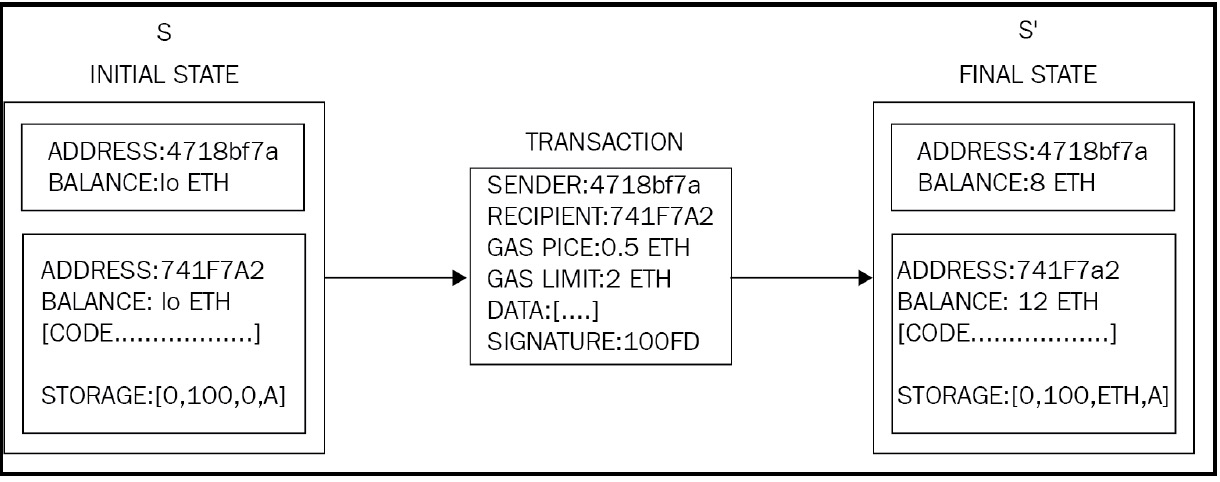
\includegraphics[width=\linewidth]{ethereum_transaction.jpg}
    \caption{Ethereum Transaction \citep{RefWorks:doc:MasteringBlockchain}}
    \label{fig:ethereum_transaction}
\end{figure}

There are currently two Ethereum networks running: Ethereum Classic (ETC) \citep{EthereumClassic} and Ethereum (ETH) \citep{Ethereum}. In this thesis, the Ethereum ETH will be used to discuss and implement the smart contract due to the speculation that the later Ethereum is more popular, advanced and actively maintained. The currency from Ethereum will be refered as "Ether" after this.

\subsection{Smart contract execution on Ethereum}

In Ethereum, each smart contract has its own address after being released to the network. To run one, an user with another Ethereum address will need to initiate a transaction to the contract, which optionally contains the amount of Ether to transfer, the message to invoke some function on the smart contract, and amount of fee (GAS) to be paid for the miners. The transaction will be verified by the network which consumes GAS gradually and if the transaction is invalid, the remaining fee will be refunded to the sender. Otherwise, the amount of Ether specified will be transfer and the code invocation will be activated on the transaction, which will run a specified function on the smart contract.